\documentclass[a4paper, oneside, openany, dvipsnames, table]{article}
\usepackage[utf8]{inputenc}


\usepackage{lmodern}
\usepackage{breakurl}
\usepackage[T1]{fontenc}
\usepackage[italian]{babel}
\usepackage{stile}
\usepackage{hyperref}
\usepackage{graphicx} 


\begin{document}
\copertina
\tableofcontents
\newpage
\section{Introduzione}
	Il seguente documento è un'analisi di usabilità del sito: \\
	\begin{center}
		\url{https://www.uniba.it/ricerca/dipartimenti/informatica/dipartimento-di-informatica}
	\end{center} 
In questa analisi verrà valutata solo la versione \textit{desktop} del sito.
  %può anche rimanere vuoto
	\subsection{Nome}
		Aggiungere immagine con nome del sito?\\
\\ 
Il nome del sito ha un impatto importante (mediamente il 10-20\% in termini di usabilità) e va quindi scelto con cura.\\
Esso deve essere incisivo, facile da ricordare e evocativo rispetto il contenuto che propone. Affinché sia evocativo è bene utilizzare parole di uso comune e che evitino qualsiasi tipo di fraintendimento nell'utente.\\
Nel nostro caso il sito è abbastanza esplicativo rispetto al contesto in cui ci troviamo (dipartimento di Informatica dell'università di Bari), nonostante vi sono alcuni particolari che non lo rendono ottimale:
	\begin{itemize}
		\item \textbf{Presenza di trattini}: in generale non apprezzati all'interno del nome da parte degli utenti;
		\item \textbf{Lunghezza}: il nome è molto lungo, quindi difficile da ricordare;
		\item \textbf{Dominio}: non è \textit{.org}, come è auspicabile che sia;
		\item \textbf{Presenza parole inusuali}: la sigla \textit{Uniba}, che rappresenta l'Università di Bari, potrebbe creare fraintendimenti 												 da parte dell'utente medio, che non necessariamente ne conosce il significato.
	\end{itemize}
In generale, quindi, il nome del sito da un'idea spannometrica del contesto in cui siamo, ma vi è un ampio margine di miglioramento sotto questo punto di vista.
	\subsection{Funzioni principali del sito}
		Il sito rappresenta il Dipartimento della facoltà di informatica dell'Università di Bari. \\
Il sito è statico, e le principali funzioni sono di carattere informativo. 
	\subsection{Utenza}
		Essendo un sito riguardante l'ambito universitario, l'utenza finale sarà prettamente composta da:
	\begin{itemize}
		\item Studenti frequentanti la Facoltà;
		\item Professori;
		\item Utenti generici in cerca di informazioni in merito alla Facoltà (per esempio futuri studenti interessati a iscriversi).
	\end{itemize}
Mentre per le prime due categorie si può supporre che essi abbiano abbastanza familiarità con il sito in questione, per quanto riguarda invece l'ultima categoria di utenti si può assumere il contrario. \\
Pertanto si può concludere che il tipo di utenza finale non sarà necessariamente specializzata e quindi vanno considerati accorgimenti a riguardo. Per esempio il linguaggio utilizzato all'interno delle pagine dovrà essere chiaro e sintetico; il contenuto dovrà essere esposto attraverso una struttura chiara, in modo che l'utente che visita per la prima volta il sito possa individuare con facilità le varie sezioni e cosa esse trattano. \\
In fase di analisi strutturale verranno analizzati questi aspetti.
	\subsection{Serach Engine Optimization}
		Con \textit{Search Engine Optimization} si intendono tutte quelle attività finalizzate ad ottenere la migliore rilevazione, analisi e lettura del sito web da parte dei motori di ricerca attraverso i loro spider, grazie ad un migliore posizionamento. \\
Il posizionamento di una pagina web è determinato da un "punteggio" ad essa assegnato, detto pagerank.\\
Il pagerank di un sito viene stabilito sulla base due due componenti: la parte testuale e quella ipertestuale.
Al fine di aumentare i punteggi relativi alle parti testuali e ipertestuali esistono diverse tecniche.
Per quanto riguarda la parte testuale si parla della tecnica di \textit{term spam}, che in sostanza consiste nel spammare keyword associate alla pagina web in determinate parti del sito. Ecco dove è preferibile spammare le keyword:
\begin{itemize}
		\item \textsc{Body della pagina}: in generale non bisogna esagerare con questa tecnica, poichè non è molto gradita dall'utente e in 						 generale rischia di intaccare il contenuto della pagina. Nel nostro caso non è praticamente utilizzata questa tecnica;
		
		\item \textsc{Tag meta}: inserendo le keyword nei metatag del sito. Le keyword dovrebbero rispecchiare la maggior parte delle 								 ricerche,costituendo un insieme coeso e di dimensione ridotta. 
					 Nel nostro caso all'interno della pagina HTML del sito non vengono inseriti alcuni tag meta, e questo è un 										grosso punto a sfavore in termini di SEO. Sarebbe stato aspicabile inserire, per esempio, le seguenti keyword: 									\\
						\begin{center}
								Informatica, Uniba, Università, Dipartimento
						\end{center}
						
		\item \textsc{Title spam}: consiste nell'inserire keyword nel tag <title>. Nel nostro caso il tag <title> è
								\\
								\begin{center}
									<title>Dipartimento di Informatica </title>
								\end{center}	
								Il tag quindi è stato utilizzato opportunamente.	
								
		\item \textsc{All'interno di link}: ovvero all'interno dei tag <a> di HTML. Questa tecnica non è utilizzata, ed è un punto a sfavore 						 poichè questa tecnica produce punteggi speciali, in quanto un link è visto come un testo "speciale", più visibile.
		
		\item \textsc{URL spam}: si tratta di inserire le keyword all'interno dell'URL. Attraverso questa tecnica si ottengono bonus simili a 						 quelli del punto precedente. Nel nostro caso nell'url sono inserite keyword adatte, quindi si può dire che la tecnica è 						 stata utilizzata correttamente. 

\end{itemize}

Per quanto riguarda la parte ipertestuale, invece, il punteggio associato è direttamente proporzionale al numero di link entranti e uscenti. Per quanto riguarda i primi non abbiamo gli strumenti per poter arrivare a conclusioni; per quanto riguarda gli outlinks, invece, si nota che sono molto numerosi (in particolare nella homepage), e questo è un aspetto positivo.\\

Alla luce di queste osservazioni analizziamo il posizionamento \textit{SERP} della pagina web.\\
Utilizzando il motore di ricerca google si eseguono delle ricerche di test per valutare la posizione del sito all'interno dei risultati:
	\begin{itemize}
		\item Dipartimento informatica: 16 posto;
		\item Uniba informatica: 1 posto;
		\item Bari informatica: 1 posto;
		\item Aldo Moro informatica: 1 posto (Aldo Moro è il nome dell'università);
		\item Informatica puglia: 19 posto;
		\item Dipartimento informatica Puglia: 2 posto;
	\end{itemize}
Considerando che il 95 per cento dei click dell'utente vanno ai primi 10 risultati, il sito si posiziona bene per ricerche specifiche, mentre con keyword di carattere più generale scende in posizioni molto basse.



		
	
	
\newpage
\section{Analisi strutturale del sito}
	\input{sez/Analisi.tex}
	\subsection{Struttura generale del sito}
		Il sito è strutturato nel seguente modo, partendo dall'alto e scendendo verso il basso:
	\begin{itemize}
		\item \textbf{Menu orrizontale con barra di ricerca}: sulla parte sinistra vi è un menu a schede, non appartenente al sito della facoltà di informatica ma all'ateneo UniBa. A prima lettura questo non è chiaro e può creare ambiguità. Inoltre un altro errore consiste nel fatto che non viene sfruttato al meglio l'angolo in alto a sinistra (punto di entrata dell'occhio dell'utente), dove sarebbe opportuno mettere il logo della facoltà. Per quanto riguarda la posizione della barra di ricerca, sulla destra, è buona. Le funzionalità della barra di ricerca verranno analizzate in una sezione dedicata sucessiva.
\begin{center}
\begin{figure}[h!]
           \begin{center}
           
\includegraphics[scale=0.40]{C:/Users/elepo/Desktop/UNI/WIM/ANALISI_SITO/Relazione/sez/Analisi/1.png}
           \caption{Menu orrizontale con barra di ricerca}
           \end{center}
  \end{figure}
\end{center}
		\item \textbf{Header}: contiene il logo della facoltà e la sua dicitura;
		\begin{center}
\begin{figure}[h!]
           \begin{center}
           
\includegraphics[scale=0.40]{C:/Users/elepo/Desktop/UNI/WIM/ANALISI_SITO/Relazione/sez/Analisi/2.png}
           \caption{Header}
           \end{center}
  \end{figure}
\end{center}
		\item \textbf{Pagina principale}: strutturata nel seguente modo:
			\begin{itemize}
				\item Parte sinistra: dedicata alle sezioni di seguito analizzate nelle sezioni di strutturazione dei contenuti, contatto con i social (facebook e twitter), login dell'area riservata del personale del dipartimento, una sezione riguardante la fatturazione elettronica (di cui personalmente non ho compreso il significato):
\begin{figure}[!htb]
   \begin{minipage}{0.48\textwidth}
     \centering
     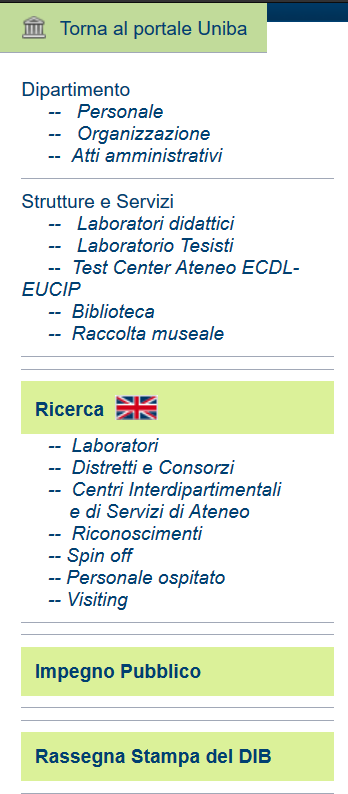
\includegraphics[width=.7\linewidth]{C:/Users/elepo/Desktop/UNI/WIM/ANALISI_SITO/Relazione/sez/Analisi/311.png}
     \caption{Parte sinistra 1}
   \end{minipage}\hfill
   \begin{minipage}{0.48\textwidth}
     \centering
     
\includegraphics[width=.7\linewidth]{C:/Users/elepo/Desktop/UNI/WIM/ANALISI_SITO/Relazione/sez/Analisi/312.png}
     \caption{Parte sinistra 2}
   \end{minipage}
\end{figure}	
		
		
		
		
		
		
		
		
		

\newpage
				\item Parte centrale: nella parte superiore troviamo informazioni generali sul dipartimento (indirizzo, direttore, coordinatore) mentre nella parte sottostante diverse sezioni dedicate a eventi, news
				\begin{center}
\begin{figure}[h!]
           \begin{center}
           
\includegraphics[scale=0.40]{C:/Users/elepo/Desktop/UNI/WIM/ANALISI_SITO/Relazione/sez/Analisi/321.png}
           \caption{Parte centrale 1}
           \end{center}
  \end{figure}
\end{center}
\begin{center}
\begin{figure}[h!]
           \begin{center}
           
\includegraphics[scale=0.40]{C:/Users/elepo/Desktop/UNI/WIM/ANALISI_SITO/Relazione/sez/Analisi/322.png}
           \caption{Parte centrale 2}
           \end{center}
  \end{figure}
\end{center}
\newpage
				\item Parte destra: riservata alle sezioni del sito in lingua inglese, didattica, due sezioni per master, portale di login per gli studenti della facoltà, informazioni generali sulla segreteria didattica
\begin{figure}[!htb]
   \begin{minipage}{0.48\textwidth}
     \centering
     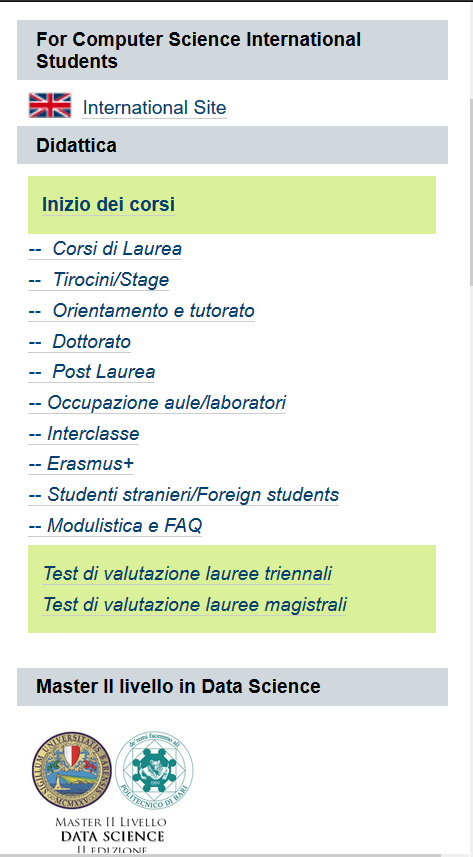
\includegraphics[width=.7\linewidth]{C:/Users/elepo/Desktop/UNI/WIM/ANALISI_SITO/Relazione/sez/Analisi/331.png}
     \caption{Parte destra 1}
   \end{minipage}\hfill
   \begin{minipage}{0.48\textwidth}
     \centering
     
\includegraphics[width=.7\linewidth]{C:/Users/elepo/Desktop/UNI/WIM/ANALISI_SITO/Relazione/sez/Analisi/332.png}
     \caption{Parte destra 2}
   \end{minipage}
\end{figure}					
				
				
				
				
			
			\end{itemize}
		\item \textbf{Footer}: si colloca nella parte inferiore della pagina e contiene contatto con i social (di nuovo), sezioni di diversa natura e le solite informazioni contenute in questa sezione.
		\begin{center}
\begin{figure}[h!]
           \begin{center}
           
\includegraphics[scale=0.40]{C:/Users/elepo/Desktop/UNI/WIM/ANALISI_SITO/Relazione/sez/Analisi/4.png}
           \caption{Footer}
           \end{center}
  \end{figure}
\end{center}
			
	\end{itemize}
\newpage




Il sito analizzato fa parte della pagina web dedicata all'Ateneo dell'università di Bari. \\
Arrivati alla homepage del sito dedicato al Dipartimento di Informatica esistono sottosezioni dedicate per soddisfare diverse esigenze.
Le principali sottosezioni che si individuano sono le seguenti:
	\begin{itemize}
		\item \textbf{Dipartimento}: contiene informazioni sul personale, organizzazione del dipartimento (consiglio, giunta, coordinatore..) e 		lo storico dell'attività amministrativa;
		\item \textbf{Strutture e servizi}: all'interno della quale sono elencate le infrastrutture (per esempio laboratori);
		\item \textbf{Ricerca}: dove troviamo tutte le informazioni relative all'attività di ricerca del Dipartimento;
		\item \textbf{Impegno pubblico}: dove sono esposte le iniziative di carattere culturale e sociale del Dipartimento;
		\item \textbf{Rassegna stampa del dipartimento};
		\item \textbf{Didattica}: dove compaiono tutte le informazioni riguardanti il corso di studi;
		\item \textbf{I nostri eventi};
		\item \textbf{Primo piano};
		\item \textbf{Le nostre notizie};
		\item \textbf{Job placement};
		\item \textbf{Master II livello in Data Science};
		\item \textbf{Short Master in Responsabili della Protezione dei Dati Personali};
		\item \textbf{Studenti@dib};
		\item \textbf{For Computer Science International Students}: sito in versione inglese.
	\end{itemize}
La strutturazione delle sezioni è molto caotica: vengono utilizzati diversi pattern visivi per sottosezioni che logicamente sembrerebbero essere della stessa entità, creando confusione nell'utente in merito alla gerarchia delle sezioni.\\
Sono stati individuati 4 tipi di pattern differenti:
	\begin{itemize}
		\item \textbf{Testo semplice blu}: vedi sezione "Dipartimento", "Strutture e servizi";
		
		\item \textbf{Testo blu grassetto su sfondo verde}: per le sezioni "Ricerca" (affiancata da una bandiera inglese di cui non si capisce 						  il senso), "Impegno pubblico", "Rassegna stampa", 
		\item \textbf{Testo blu grassetto sottolineato in grigio su sfondo verde}: si trova nella sotto-sezione "Inizio dei corsi";
		\item \textbf{Testo blu corsivo sottolineato in grigio su sfondo verde}: si trova nelle sotto-sezioni riguardanti i test di 								  valutazione;
		\item \textbf{Testo nero grassetto su sfondo grigio}: per la sezione "Didattica", "Primo piano", "I nostri eventi", "Le nostre 								  notizie", "Job placement", "Studenti @dib", "Short Master in responsabili della protezione dei dati personali"; "Master 						  in data science", "For Computer Science International Students". Inoltre in queste sezioni esiste ancora più incongruenza, dal momento che alcune di queste sono cliccabili ("Le nostre notizie", "in primo piano", "i nostri eventi") con testo che diventa verde quando ci si passa sopra con il cursore, altre non sono cliccabili ma contengono sottosezioni riportate sotto forma di elenchi cliccabili e altre ancora non hanno sottosezioni riportate sotto forma di elenco, ma hanno delle immagini cliccabili che riportano al sito dedicato ("Master II livello in Data Science" e "Short Master in Responsabili della Protezione dei Dati Personali").
	\end{itemize}
Inoltre esistono anche tre pattern differenti per indicare le sottosezioni incluse nelle sezioni precedentemente elencate:
	\begin{itemize}
		\item \textbf{Testo corsivo blu preceduto da doppi trattini}: per gli elenchi appartenenti alle sezioni "Dipartimento", "Strutture e servizi" e "ricerca". Quando si passa sul cursore sul testo non accade nulla;
		\item \textbf{Testo corsivo blu sottolineato grigio preceduto da doppi trattini}: per gli elenchi appartenenti alla sezione "Didattica". Quando si passa sul cursore sul testo diventa verde;
		\item \textbf{Testo corsivo blu sottolineato grigio senza trattini}: per gli elenchi appartenenti alla sezione "Studenti @dib". Quando si passa sul cursore sul testo diventa verde.
	\end{itemize}

In linea teorica è corretto utilizzare pattern differenti per esibire sezioni di diversa importanza, ma bisogna fare attenzione nell'usare questa tecnica onde evitare di impedire all'utente di fare uno scanning corretto del sito. \\
Nel sito in esame il risultato è disastroso: si privilegiano e mettono in primo piano contenuti di importanza secondaria (vedi sezione "Rassegna stampa del Dib") e le sezioni di uguale importanza (per esempio "Didattica" e "Strutture e servizi", entrambi di carattere informativo in merito alle strutture e alle opportunità offerte dall'ateneo) sono evidenziate con pattern differenti.\\
Inoltre vi è un senso di incongruenza generale che peggiora ancora di più l'impatto visuale, come se le diverse sezioni fossero state incollate tra di loro senza un minimo di criterio.\\
Un altro aspetto negativo consiste nel fatto che le diverse sezioni non sono organizzate all'interno di un menù che le contenga tutte, ma sono distribuite in maniera del tutto casuale all'interno della pagina (a sinistra, a destra, nella parte centrale). Vi è una forte dispersione.\\
Infine va sottolineato che il menù in alto a destra nella pagina non è relativo al sito del dipartimento di informatica, ma all'ateneo UniBa, quindi in questa analisi non verrà citato. Si sottolinea solamente che non è scontato supporre che l'utente sappia che le voci del menù in alto reindirizzano al sito UniBa, e questo potrebbe scaturire confusione.




	\subsection{Organizzazione dell'informazione}
		
Oltre al pessimo impatto visuale anche i contenuti delle sezioni sono organizzate in maniera confusionaria: non vi è una buona separazione dei contenuti. Per esempio la voce "occupazione aule e laboratori" compare nella sezione "Didattica" e non all'interno di "strutture e servizi", come logicamente dovrebbe essere.\\
Inoltre le varie sezioni non sono mutamente esclusive (vedi "In primo piano" e "I nostri eventi", non cambia nulla), creando una forte ridondanza.\\
Inoltre per la maggior parte delle sezioni le relative sotto parti sono visibili grazie all'esposizione tramite elenco puntato, mentre per altre (vedi "Job placement") bisogna cliccare sul titolo della sezione e solo in seguito si viene indirizzati a una pagina contenente le sottosezioni. Questo in fase di scanning potrebbe causare molta confusione: l'utente potrebbe essere indotto a pensare che, per esempio, la sezione "Job placement" non abbia sotto sezioni (anche perchè primo non è scontato che il titolo sia cliccabile, visto che da altre parti con lo stesso pattern non lo è, e secondo perchè vi è già esposto del contenuto, quindi si potrebbe pensare che la struttura della sezione si limiti a riportare il contenuto). \\
In conclusione la strutturazione del contenuto non è per niente intuitiva, probabilmente sono necessari svariati click per permettere all'utente di arrivare all'informazione voluta e la strutturazione dei contenuti nelle pagine interne è ambigua.

	\subsection{Parti salienti}
		Le sezioni più importanti che il sito propone:
	\begin{itemize}
		\item \textbf{Didattica}: di carattere informativo;
		\item \textbf{Studenti @dib}: portale per gli studenti iscritti alla facoltà;
		\item \textbf{Dipartimento}: di carattere informativo.
	\end{itemize}
Il resto delle sezioni, seppure riportate allo stesso livello di importanza di quelle sopra elencate sono (a mio parere) secondarie o comunque incluse nelle sezioni sopra citate.
	

\newpage
\section{Homepage}
	\input{sez/Homepage.tex}
	\subsection{Descrizione}
		La homepage è la vetrina del sito, deve dare una chiara idea del contenuto delle pagine interne e soprattutto fornire all'utente tutte le informazioni necessarie in
modo chiaro e nel minor tempo possibile.\\
In generale la strutturazione dell'homepage non è molto chiara, dal momento che le varie sezioni riportano diversi tipi di informazioni, molto eterogenee tra di loro.\\
Un altro aspetto negativo consiste nel fatto che per visualizzare l'intera homepage è necessario effetuare almeno due scroll.\\

	\subsection{Le 6 w}
		\input{sez/Homepage/Le6w.tex}
		\subsubsection{Where}
			Asse che risponde alla domanda: dove mi trovo? A che tipo di sito sono arrivato? Che contenuto viene offerto? \\
Il primo posto in cui può essere reperita l'informazione è l'header, nella quale la presenza di un logo è di vitale importanza. In questo caso il logo non è posizionato nell'angolo in alto a sinistra all'interno dell'header; sebbene non sia nella posizione ottimale è comunque abbastanza visibile ed è in grado di indicare all'utente che si tratta del sito riguardante la facoltà di informatica dell'università Aldo Moro.\\
In seguito l'utente ha ulteriori informazioni in merito al contenuto del sito facendone un paio di scroll.

		\subsubsection{Who}
			Asse che risponde alla domanda: chi rappresenta questo sito?  \\
Come detto precedentemente, il logo sebbene non posizionato in maniera ottimale è comunque abbastanza visibile, ed è quindi in grado di rispondere alla domanda. \\
Ulteriori chiarimenti in merito si possono ottenre consultando il footer della pagina (il cui difetto è però essere reperibile solo attraverso una serie di scroll da parte dell'utente).
		\subsubsection{Why}
			Asse che risponde alla domanda: che benefici mi offre il sito? Perchè dovrei rimanere? \\
Nel nostro caso si tratta di un sito senza "competitori" dal momento che è la pagina riguardante una facoltà universitaria di un determinato ateneo. Per questo la pagina in sè non ha il bisogno di indicare esplicitamente quali vantaggi offre il sito, dal momento che comunque è l'unico sito disponibile per offrire tale informazione. \\
Ciò non toglie che esporre le agevolazioni e i punti di forza che il sito offre sarebbe un aspetto positivo, che però la pagina in analisi non indica.
		\subsubsection{What}
			Asse che risponde alla domanda: che cosa offre questo sito? \\
La homepage risponde (seppure in modo molto disordinato) alla domanda, dal momento che vengono presentate le varie opzioni che l'utente ha quando arriva alla pagina: può informarsi in merito al corso di studi, può entrare nell'area riservata, può consultare la bacheca eventi/news e via dicendo. \\
Da sottolineare però il fatto che la tipologia di pagina aiuta alla risposta di questa domanda: il fatto che si tratti della pagina relativa a un corso di studi è abbastanza autoesplicativa rispetto al suo contenuto. A mio avviso se un sito commerciale adottasse la stessa strutturazione dei contenuti la homepage non sarebbe in grado di dare informazioni rispetto quest'asse, quindi l'essere in grado di soddisfare l'asse a mio avviso è garantito unicamente dalla natura della pagina stessa e non dalla strutturazione del suo contenuto.
		\subsubsection{When}
			Asse che risponde alla domanda: quando è stato aggiornato il sito? Quali sono le novità rispetto il mio ultimo accesso? \\
Il sito è in grado di rispondere alla domanda dal momento che nella parte centrale viene indicata la data di ultima modifica. \\
%IMMAGINE??
L'aspetto negativo, però, è che la data riportata per le ultime modifiche risale a un periodo molto lontano (un anno circa). Considerando che la pagina possiede una bacheca eventi, una data del genere lascia perplessi: si suppone quindi che da un anno a questa parte non sia stato organizzato nessun evento relativo al corso? Improbabile. L'ipotesi più ragionevole è quella di pensare che il sito non sia stato aggiornato regolarmente. Questo da una sensazione di staticità molto negativa, che porta l'utente a pensare che probabilmente il sito non ha contenuti aggiornati in grado di rispondere in modo corretto alle sue richieste.
		\subsubsection{How}
			Asse che risponde alla domanda: come arrivo alle sezioni principali del sito? \\
Analizzando i seguenti aspetti:
	\begin{itemize}
		\item Che tipo di menù abbiamo? Per tutti i menù esistenti abbiamo menù a schede, un layout molto comune che rende facile capire che quell'elemento è un menù;
		\item Il menù è facile da individuare? Si, si è in grado di capire che parti della pagina rappresentano un menù;
		\item Il numero di voci è adeguato? La risposta per tutti i menù presenti è no: sono troppe (talvolta è necessario un scroll per visualizzarle tutte), soprattutto considerando che, come già detto in precedenza, spesso il contenuto è condiviso da una o più sezioni;
		\item L'interlinea tra le voci è adeguata? No, la spaziatura verticale tra una voce e l'altra è molto bassa, e questo rende il fault-tolerance in caso di sbaglio di click molto basso.
		\item La strutturazione delle voci è chiara (per esempio esistono macro categorie)? Come detto ampiamente in precedenza, no.
	\end{itemize}
		\subsection{Note}
		Una nota negativa riguardante la homepage consiste nell'esistenza di un link circolare all'homepage: quando sono nell'homepage e clicco sul logo la pagina home viene ricaricata	
			


\newpage
\section{Pagine Interne}
	\input{sez/Pag_interne.tex}
	\subsection{Descrizione}
		La struttura delle pagine interne al sito è molto eterogenea, fattore che crea confusione e disorientamento da parte dell'utente. Infatti i layout possibili per le pagine interne (le hanno lo stesso livello di annidamento o addirittura appartengono allo stesso menù) individuati sono 3:
	\begin{itemize}
		\item Il primo, comune a tutte le voci del menù di sinistra (tranne la voce "biblioteca") e alle voci del menù in alto a destra:
\begin{center}
\begin{figure}[h!]
           \begin{center}
           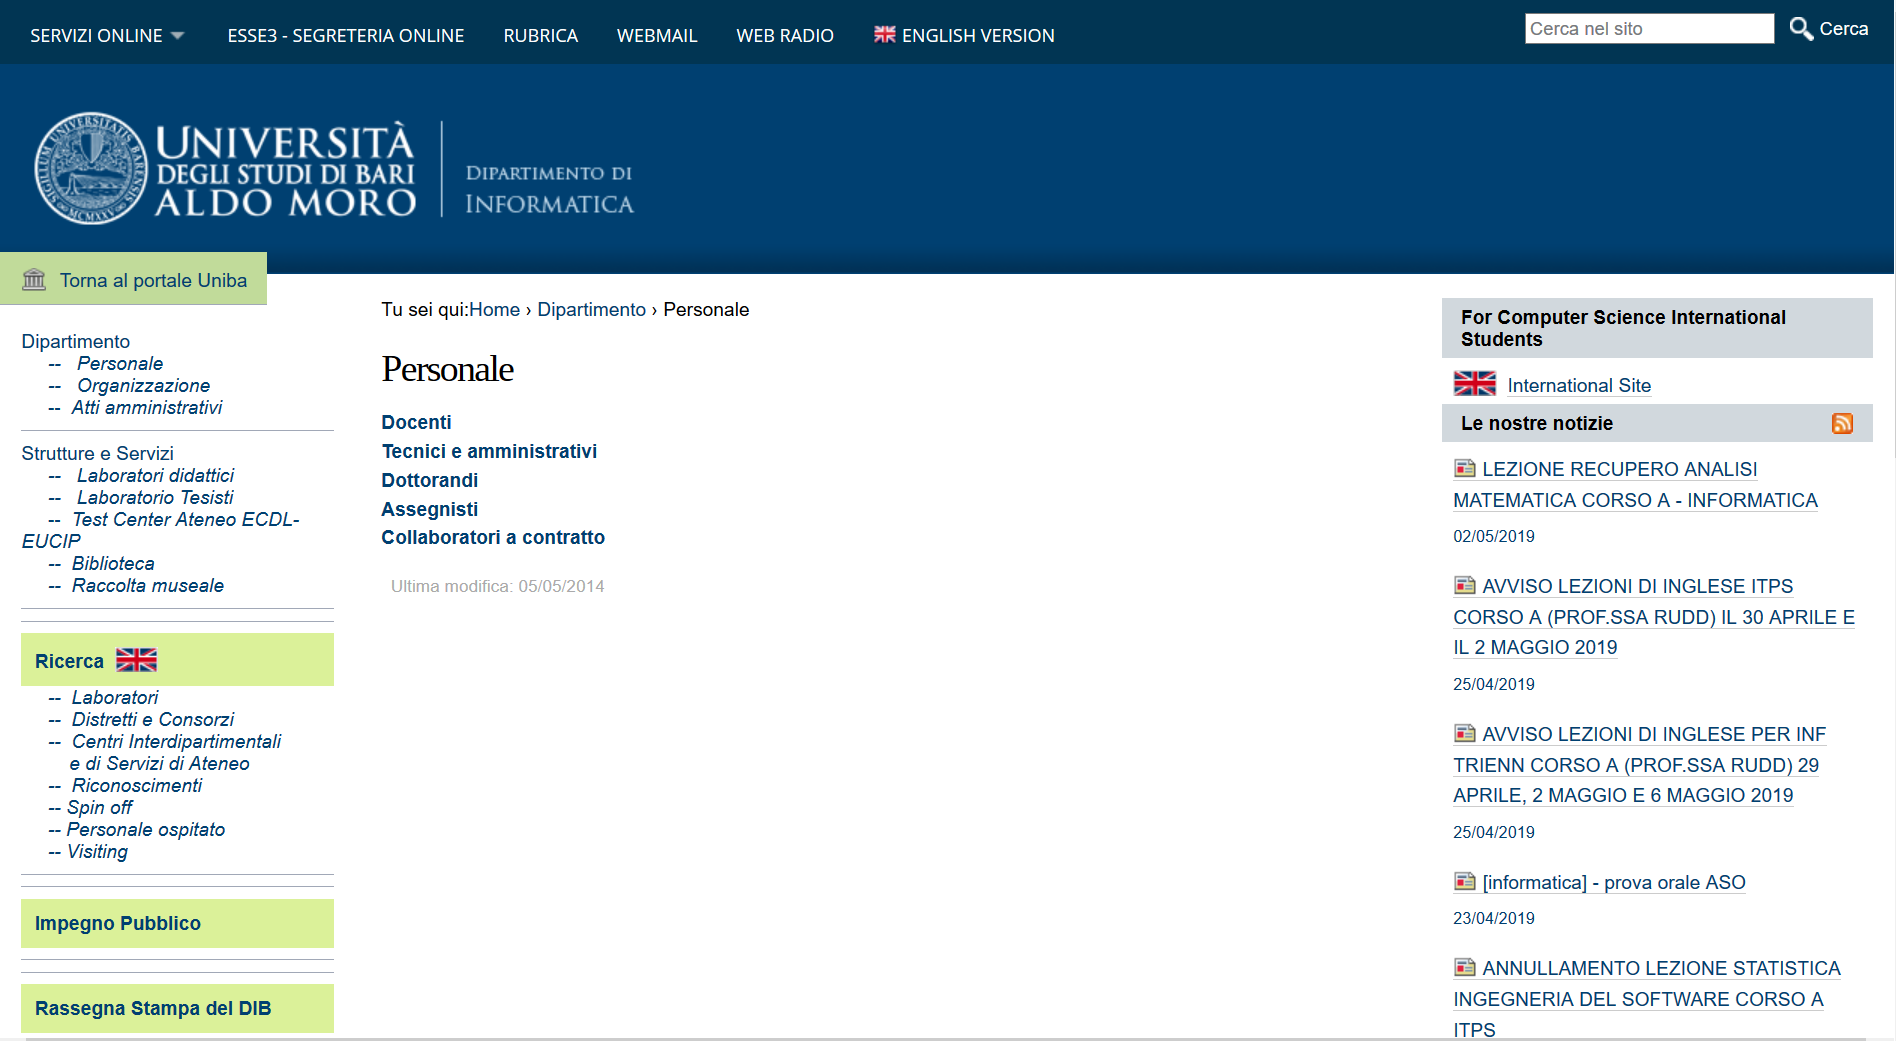
\includegraphics[scale=0.40]{C:/Users/elepo/Desktop/UNI/WIM/ANALISI_SITO/Relazione/sez/Pag_interne/layout1.png}
           \caption{Layout 1}
           \end{center}
  \end{figure}
\end{center}
		\item Un secondo layout, completamente incongruente rispetto al primo, proprio solo della voce "biblioteca" del menù di sinistra, che reindirizza al sito dell'ateneo Aldo Moro:
		\begin{center}
\begin{figure}[h!]
           \begin{center}
           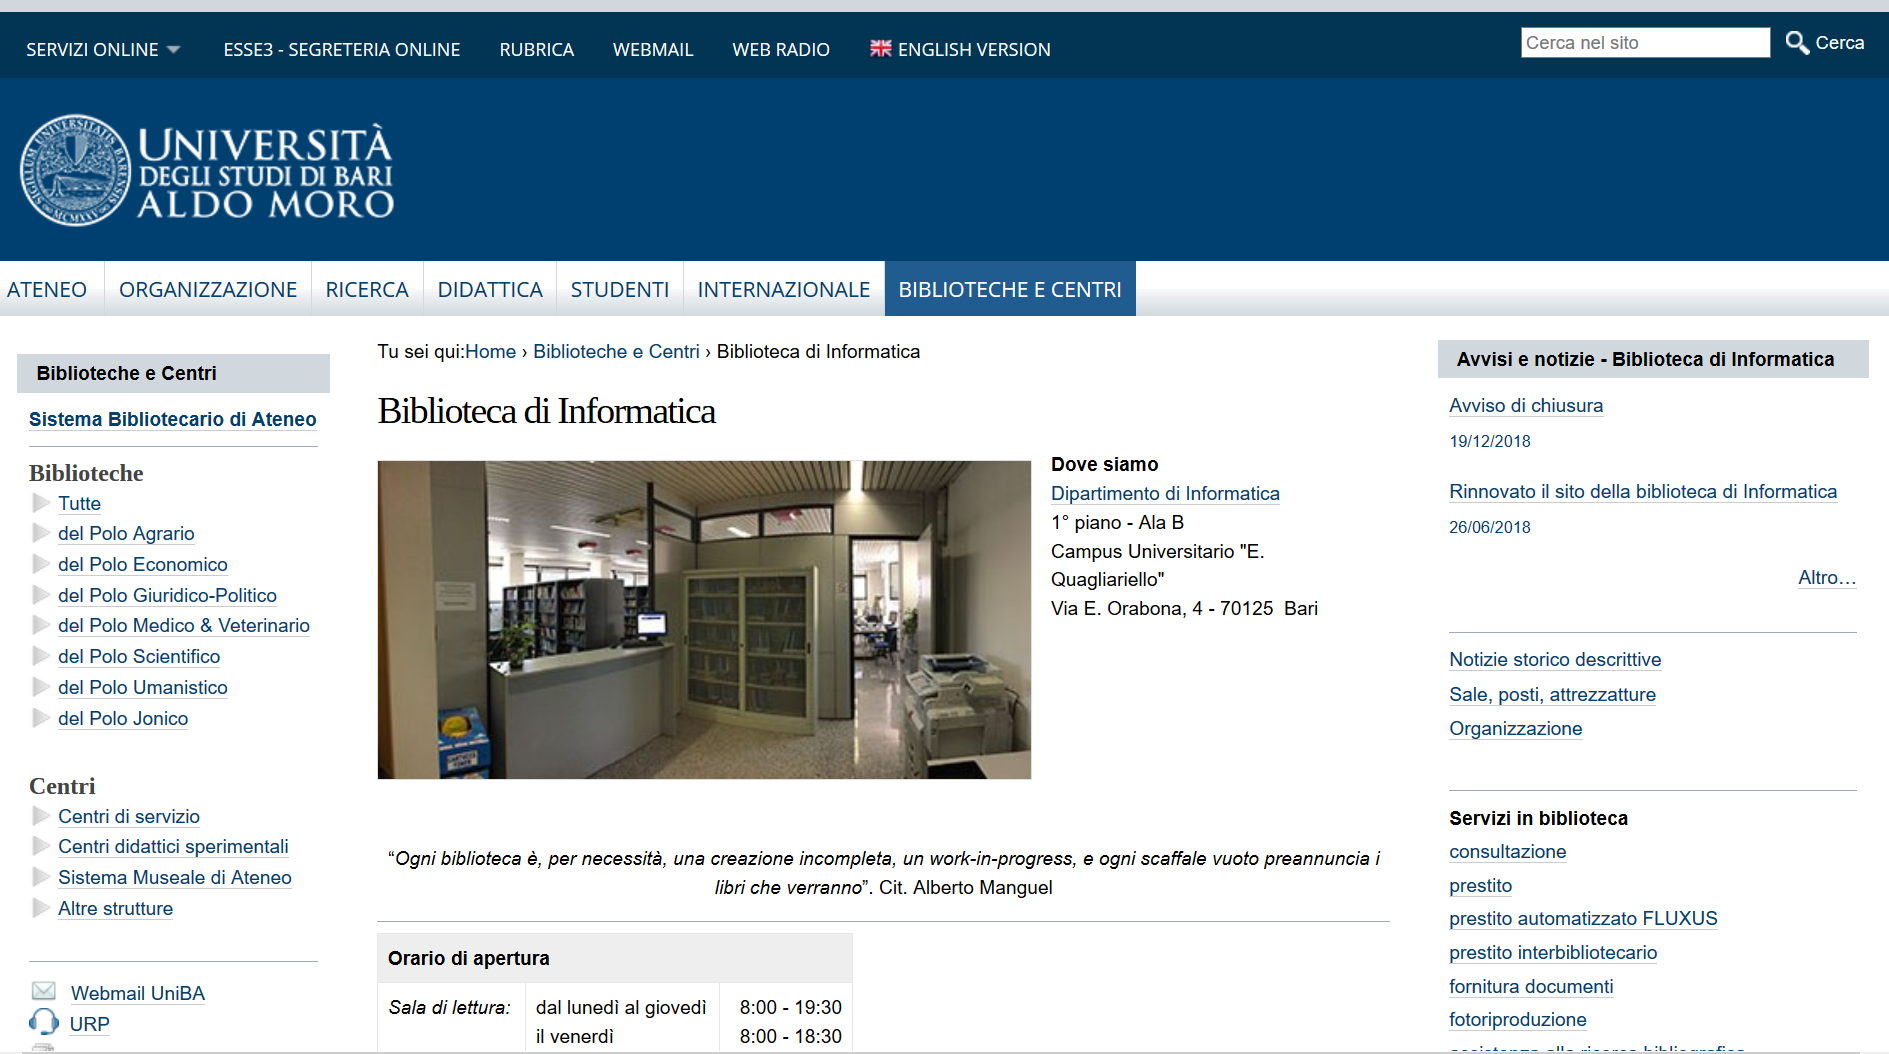
\includegraphics[scale=0.40]{C:/Users/elepo/Desktop/UNI/WIM/ANALISI_SITO/Relazione/sez/Pag_interne/layout2.png}
           \caption{Layout 2}
           \end{center}
  \end{figure}
\end{center}
\newpage
		\item Un terzo layout comune alle voci del menù di destra in basso:
		\begin{center}
\begin{figure}[h!]
           \begin{center}
           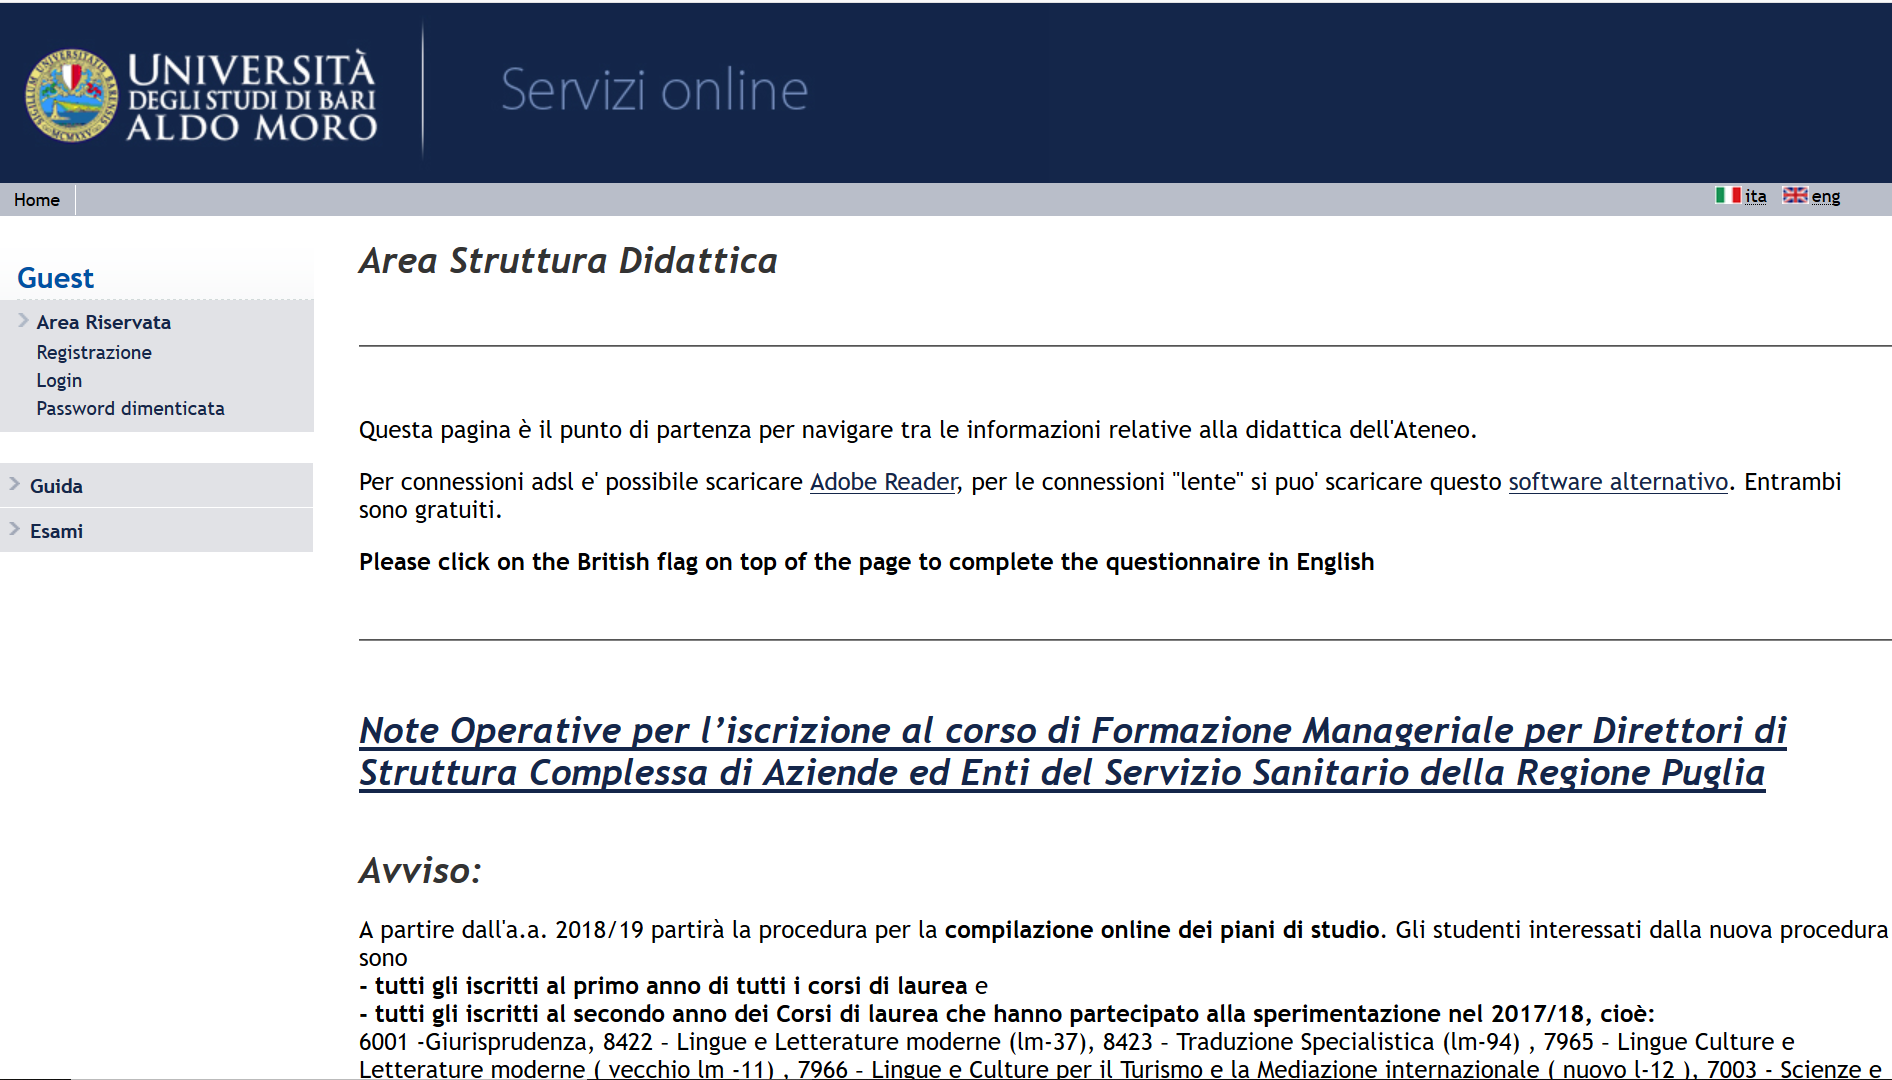
\includegraphics[scale=0.40]{C:/Users/elepo/Desktop/UNI/WIM/ANALISI_SITO/Relazione/sez/Pag_interne/layout3.png}
           \caption{Layout 3}
           \end{center}
  \end{figure}
\end{center}
	\end{itemize}
A mio avviso il fatto che una voce del menù di sinistra ("biblioteca") abbia un layout completamente differente rispetto alle voci appartenenti allo stesso menù è molto disorientante, dal momento che voce appartenenti allo stesso menù o a livelli di annidamenti analoghi dovrebbero avere lo stesso layout.\\
Un altro fattore negativo è l'utilizzo inconsistente del breadcrumb: per esempio per voci allo stesso livello di annidamento troviamo due breadcrumb totalmente differenti:

	\subsection{Come cambiano le 6 W}
		Per quanto riguarda le pagine interne di un sito web, gli assi informativi obbligatori riassunti nelle "6 w" cambiano.\\
Infatti restano obbligatori gli assi Where, Who e What, mentre diventano opzionali gli assi Why, When e How. Analizziamo in generale come le pagine interne rispondono agli assi informativi:
	\begin{itemize}
		\item \textbf{Where}: a mio avviso l'utente è difficilmente in grado di capire dove si trova, sia per l'utilizzo incongruente del breadcrumb, sia per la struttura eterogenea delle pagine interne. Questo disorientamento si accentua soprattutto per le voci dei menù che reindirizzano a pagine web di altri siti (per esempio quelli che reindirizzano al portale principale dell'ateneo Aldo Moro)\begin{center}
\begin{figure}[h!]
           \begin{center}
           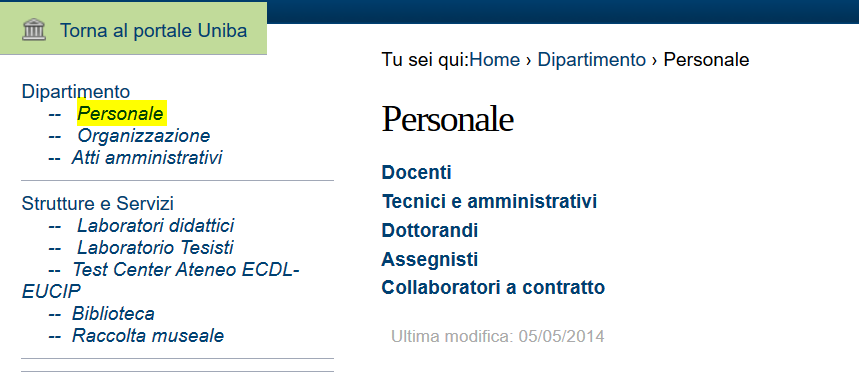
\includegraphics[scale=0.40]{C:/Users/elepo/Desktop/UNI/WIM/ANALISI_SITO/Relazione/sez/Pag_interne/b1.png}
           \caption{Breadcrumb di tipo 1}
           \end{center}
  \end{figure}
\end{center}

\begin{center}
\begin{figure}[h!]
           \begin{center}
           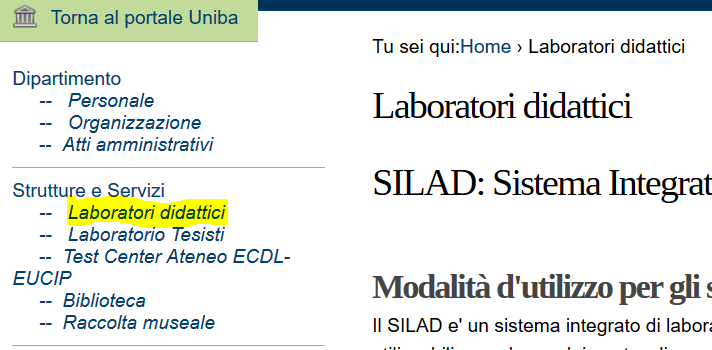
\includegraphics[scale=0.40]{C:/Users/elepo/Desktop/UNI/WIM/ANALISI_SITO/Relazione/sez/Pag_interne/b2.png}
           \caption{Breadcrumb di tipo 2}
           \end{center}
  \end{figure}
\end{center}
		\item \textbf{Who}: il logo continua a essere presente nell'header, pertanto anche a questa domanda l'utente trova una risposta;
		\item \textbf{What}: anche in questo caso il contenuto è abbastanza dichiarativo da poter rispondere alla domanda.
	\end{itemize}

Per quanto riguarda invece gli assi opzionali:
	\begin{itemize}
		\item \textbf{Why}: essendo un portale web dedicato a una struttura universitaria la pagina non ha "concorrenza" da parte degli altri siti, pertanto la pagina non è interessata a fornire alcun tipo di informazione in merito ai benefici nel suo utilizzo;
		\item \textbf{When}: La data degli ultimi aggiornamenti delle pagine interne è sempre presente e risponde all'asse informativo. Purtroppo però le date riportate per gli aggiornamenti sono molto antecedenti: questo è un fattore negativo riscontrato anche nella homepage che da un senso di staticità al sito.
		\item \textbf{How}: il come arrivare alle sottosezioni delle pagine interne o in generale come reperire una certa informazione non è per nulla chiaro a causa della eterogeneità della struttura delle pagine.
	\end{itemize}
	
	
	
		
	
\newpage
\section{Barra di ricerca}
	L'importanza della barra di ricerca all'interno di un sito web è direttamente proporzionale alla grandezza del sito: tante più pagine vi sono, più l'utente si affida alla barra di ricerca per la navigazione. \\
Nel nostro caso, il sito contiene molte pagine interne. Aggiungendo il fatto che il contenuto in esse esposte è mal organizzato, è molto probabile che l'utente medio si affidi alla barra di ricerca per orientarsi nella navigazione.\\
Partiamo dall'analisi di questo componente commentando la sua visibilità. La barra è collocata in una buona posizione (alto a destra, in conformità con molti altri siti). Graficamente essa rispecchia il tool proposto dal motore di ricerca Google, al quale l'utente è abituato: un box testuale affiancato da una lente di ingrandimento e dalla dicitura "Cerca...". La grandezza consigliata per la barra di ricerca è almeno 30 caratteri (al fine di coprire la maggior parte delle ricerche che un utente può effettuare). Nel nostro caso la barra non rispetta questa direttiva: si ferma a 23 caratteri.\\

\begin{center}
\begin{figure}[h!]
           \begin{center}
           
\includegraphics[scale=0.80]{C:/Users/elepo/Desktop/UNI/WIM/ANALISI_SITO/Relazione/sez/ricerca.png}
           \caption{Barra di ricerca}
           \end{center}
  \end{figure}
\end{center}
Per quanto riguarda invece la scelta dei colori, invece, la barra è bianca è lo sfondo dietro blu: il contrasto è abbastanza evidente e rende visibile la barra.\\
Un aspetto positivo consiste nel fatto che esiste la possibilità di effettuare una ricerca avanzata, la quale aggiunge filtri alla ricerca corrente (anno scolastico, opzioni di visualizzazione, numero di risultati per pagina).\\
\begin{center}
\begin{figure}[h!]
           \begin{center}
           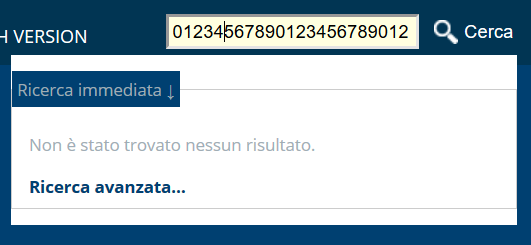
\includegraphics[scale=0.80]{C:/Users/elepo/Desktop/UNI/WIM/ANALISI_SITO/Relazione/sez/ricerca2.png}
           \caption{Ricerca avanzata}
           \end{center}
  \end{figure}
\end{center}
Una volta eseguita una ricerca (che sia basilare o avanzata non importa) i risultati sono visualizzati ad elenco, in un formato all'incirca similare a quello proposto dal motore di ricerca Google (e questo è un fattore positivo perchè l'utente ci è abituato). Un aspetto negativo, però, consiste nel fatto che se non esistono corrispondenza non viene data alcuna spiegazione o suggerimento all'utente per indirizzarlo verso una ricerca proficua.

\begin{center}
\begin{figure}[h!]
           \begin{center}
           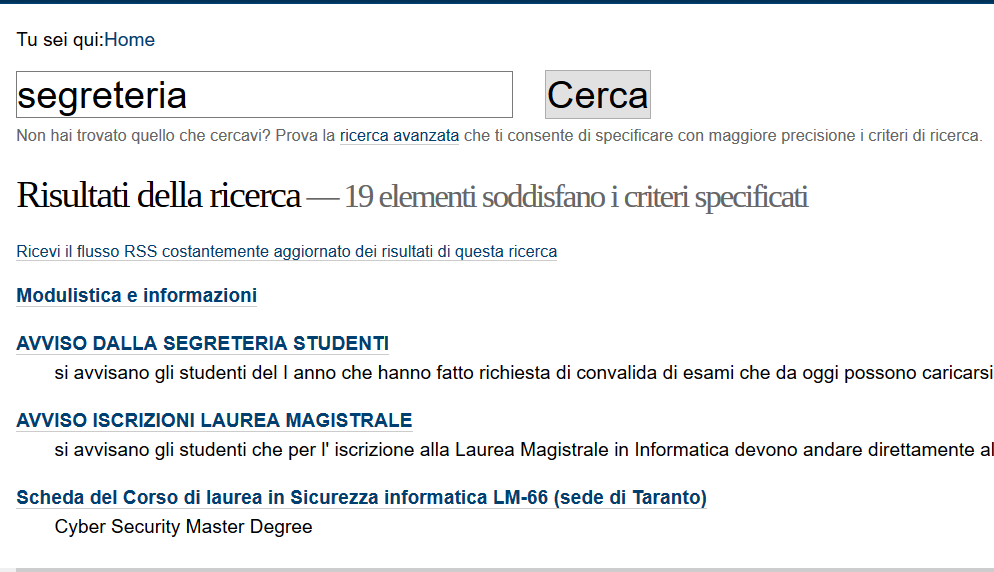
\includegraphics[scale=0.80]{C:/Users/elepo/Desktop/UNI/WIM/ANALISI_SITO/Relazione/sez/rr.png}
           \caption{Visualizzazione risultati ricerca}
           \end{center}
  \end{figure}
\end{center}
	
\newpage
\section{Contenuto}
	Analizziamo in seguito i principali componenti grafici/testuali del sito:
	\begin{itemize}
		\item \textbf{Testo}: in generale per quasi la totalità del testo esiste un adeguato contrasto tra sfondo e colore del testo, questo amplifica la visibilità dello stesso. Non vi è la possibilità di fare la resize del testo, e questo è un fattore negativo; d'altro canto esiste la possibilità di cambiare la lingua in inglese (anche se la traduzione in alcune sezioni lascia un po' a desiderare). Il testo presenta inoltre almeno tre font differenti (parlando di testo della stessa entità) e questo crea confusione e disorientamento. Inoltre, a mio avviso, il testo non è sufficientemente sintetico, anzi, e quindi non permette all'utente di individuare subito i contenuti salienti. Inoltre esso non è diviso in paragrafi e capitoli, e questo influisce negativamente in termini di timer dell'utente;
		\item \textbf{Immagini}: in generale le immagini rispettano la taglia minima consigliata (250x250 px) e sono ben visibili. Sono coerenti con il contenuto del sito (mostrano sedi, studenti che lavorano al computer e laboratori) e nel caso della homepage alleggeriscono un testo fin troppo monolitico. Inoltre esse non sono animate, e questo è un fattore positivo dal momento che il Bloated design è odiato dall'utente;
		\item \textbf{Link}: la gestione dei link (come già accennato in analisi dell'homepage) è totalmente scorretta: essi sono indicati con almeno tre diversi stili e solo uno tra essi rispetti le usuali convezioni per la segnatura dei link, questo non aiuta l'utente a individuarli con facilità. Non è inoltre possibile distinguere i link visitati da quelli no, creando ulteriore confusione. L'unico aspetto positivo è che se clicco uno di essi il suo contenuto non è visualizzato in un'altra scheda (cosa odiata dagli utenti, che amano la navigazione all'indietro) ma in quella corrente.
	\end{itemize}

	
\newpage
\section{Cose che non dovrebbero esserci..}
	Per quanto riguarda la presenza di contenuto sgradito all'utente:
	\begin{itemize}
		\item \textbf{Pop-up}: presente. Nello specifico viene aperto un pop-up che informa l'utente dell'utilizzo di cookie: \\ 
								\begin{center}
\begin{figure}[h!]
           \begin{center}
           
\includegraphics[scale=0.40]{C:/Users/elepo/Desktop/UNI/WIM/ANALISI_SITO/Relazione/sez/cookie.png}
           \caption{Cookie}
           \end{center}
  \end{figure}
\end{center}
		\item \textbf{Richieste d'uso di plugin}: non presente;
		\item \textbf{Apertura indesiderata di contenuti audio/video}: non presente;
		\item \textbf{Pubblicità}: non presente;
		\item \textbf{Registrazione forzata}: non presente.
	\end{itemize}


\newpage
\section{Giudizio finale}
	Concludendo, a mio avviso gli aspetti negativi del sito superano di gran lunga quelli positivi. Aggiungendo il fatto che si tratti di un sito di una facoltà di informatica, ritengo glie errori in termini di usabilità individuati inaccettabili.
\begin{center}
	Voto: 4
\end{center}

\newpage

	     \listoffigures
\end{document}